% !TeX program = lualatex
% ================================================================
% Polish Tier 3 Vocabulary Version of IntroducingIndicesAndRoots
%
% Generated by the server using the following settings:
%
%   language            Polish (pol)
%   text direction      left to right
%   font                Noto Serif
%   fallback font       Noto Serif
%   built from          latex/worksheets/indices/introducingIndicesAndRoots.tex
%   vocabulary key      latex/worksheets/indices/introducingIndicesAndRoots/L2/pol/introducingIndicesAndRoots_polishKey.tex
%   tier 3 vocabulary   green   RGB 0 128 0
%   English text        black   RGB 0 0 0
%   Polish text         purple  RGB 112 48 160
%   layout macros       version 3
%
% Please don't edit any information in this comment block - the server
% compares it against the current settings and rebuilds this file when
% they differ, so changes here would be overwritten. However, feel free
% to make updates to the LaTeX below if you want to edit it.
% ================================================================

\documentclass[12pt,a4paper]{article}
% ================================================================
% Copied from the English sheet this was translated from, so that
% anything it sets up for itself still works here
% ================================================================
\usepackage[a4paper,top=12mm,bottom=14mm,left=15mm,right=15mm]{geometry}
\usepackage[T1]{fontenc}
\usepackage{amsmath}
\usepackage{amssymb}
\usepackage{cancel}
\usepackage{enumitem}
\usepackage{multicol}
\usepackage{array}
\usepackage{tikz}
\usepackage[most]{tcolorbox}
\usetikzlibrary{arrows.meta}

% ================================================================
% An introduction to indices and roots.
%
% A first sheet on index notation that also builds on algebraic
% notation and on simplifying fractions. Indices are met first with
% integers and decimals, through a match-up of calculations and their
% answers, and then in context through the area of a square and the
% volume of a cube, where the root appears as the operation that
% undoes the index.
%
% The sheet then moves to algebraic variables, writing repeated
% multiplications such as a x a x a over b x b in index form and back
% again. Cancelling a factor found in both the numerator and the
% denominator is taught with integers first, then with a mix of
% integers and variables, and is then used on fractions written with
% indices in a second match-up.
%
% The extension uses the same cancelling on factorials, where most of
% the factors divide out, then asks what happens to powers and roots
% of negative numbers, and ends on the tesseract, the four-dimensional
% shape after the cube, whose corners, hypervolume and edges are all
% counted by powers of 2. Answers are on the last page.
%
% The sheet is written on, so every question is followed by a working
% area. The \newpage commands in the body are placed so that no
% question is split across the fold.
% ================================================================

\pagestyle{empty}
\linespread{1.15}\selectfont
\setlength{\parskip}{5pt}
\setlist[enumerate,1]{label=\textbf{Q\arabic*.}, leftmargin=*, itemsep=10pt, topsep=6pt, parsep=4pt}
\setlist[enumerate,2]{label=(\alph*), leftmargin=*, itemsep=8pt, topsep=5pt, parsep=3pt}
\setlength{\multicolsep}{4pt}
\setlength{\parindent}{0pt}

\newcommand{\ansline}[1][2.2cm]{\underline{\hspace{#1}}}
% A short gap for a single number, sized to sit inside a line of maths.
\newcommand{\gap}{\underline{\hspace{0.7cm}}}
% A gap for a number that is written as an index, or on the top or the
% bottom of a fraction. An underline sits too low to be read as an
% index, so a faint dotted box marks where the number is written. The
% size is given in points so that the box does not shrink away when it
% is set as an index.
\newcommand{\boxgap}[1][9pt]{\tikz[baseline=-0.8pt]\draw[gray!60,densely dotted,thick]
  (0,0) rectangle (#1,#1);}

% A worked example: the method shown in full before it is practised.
% The boxes are tinted only faintly, and their title bars are pale with
% coloured text rather than solid, so that the sheet is cheap to print.
\newtcolorbox{wex}[1]{colback=blue!1,colframe=blue!45!black,boxrule=0.6pt,
  colbacktitle=blue!8,coltitle=blue!50!black,
  left=6pt,right=6pt,top=4pt,bottom=5pt,
  title={\bfseries\small Worked example: #1},fonttitle=\small,
  toptitle=1pt,bottomtitle=1pt}

% The idea a section is built on, stated once and boxed.
\newtcolorbox{keyidea}{colback=orange!2,colframe=orange!60!black,boxrule=0.6pt,
  left=6pt,right=6pt,top=4pt,bottom=4pt}

% The notation for a section, set out so that it can be found again
% from anywhere on the sheet.
\newtcolorbox{notation}[1]{colback=green!1,colframe=green!35!black,boxrule=0.9pt,
  colbacktitle=green!10,coltitle=green!30!black,
  left=8pt,right=8pt,top=5pt,bottom=5pt,
  title={\bfseries Notation: #1},fonttitle=\normalsize,
  toptitle=2pt,bottomtitle=2pt}

% A warning about a mistake that is easy to make.
\newtcolorbox{warning}{colback=red!2,colframe=red!55!black,boxrule=0.6pt,
  left=6pt,right=6pt,top=4pt,bottom=4pt}

% The section headings, kept tight so the parts do not eat the page.
\newcommand{\heading}[1]{%
  \vspace{2pt}
  {\color{blue!45!black}\rule{\linewidth}{1pt}}\\[1pt]
  {\large\bfseries #1}\\[-6pt]
  {\color{blue!45!black}\rule{\linewidth}{0.4pt}}
  \vspace{2pt}}
\newcommand{\parttitle}[2]{\heading{Part #1: #2}}

% ----------------------------------------------------------------
% A match-up: calculations in a numbered column on the left, answers in
% a lettered column on the right, with a gap between them for the lines
% pupils draw. The answers are deliberately out of order.
% \matchup[<row spacing>][<column gap>]{<left items>}{<right items>}
% Each item is written inside braces so that it counts as one item.
\newcommand{\mletter}[1]{\ifcase\numexpr#1\relax\or A\or B\or C\or D\or E\or
  F\or G\or H\or I\or J\fi}
\NewDocumentCommand{\matchup}{O{1.1} O{7.2} +m +m}{%
\par\vspace{2pt}\noindent\hfil
\begin{tikzpicture}[mbox/.style={draw=blue!45!black,rounded corners=3pt,thick,
    fill=white,minimum width=2.9cm,minimum height=0.9cm,inner sep=3pt}]
  \foreach [count=\i from 1] \l in {#3} {%
    \node[mbox] (mL\i) at (0,{-#1*\i}) {\l};
    \node[font=\small\bfseries,anchor=east] at ([xshift=-5pt]mL\i.west) {\i.};}
  \foreach [count=\j from 1] \r in {#4} {%
    \node[mbox] (mR\j) at (#2,{-#1*\j}) {\r};
    \node[font=\small\bfseries,anchor=west] at ([xshift=5pt]mR\j.east) {\mletter{\j}};}
\end{tikzpicture}%
\hfil\par\vspace{2pt}}

% ----------------------------------------------------------------
% A 3 by 3 grid of unit squares, which is what 3 squared counts.
\newcommand{\squarepic}{%
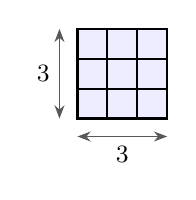
\begin{tikzpicture}[scale=0.38]
  \foreach \x in {0,1,2} \foreach \y in {0,1,2}
    \draw[thick,fill=blue!7] (\x,\y) rectangle ++(1,1);
  \draw[<->,>=Stealth,gray!70!black] (0,-0.6) -- (3,-0.6)
    node[midway,below,font=\small,black] {$3$};
  \draw[<->,>=Stealth,gray!70!black] (-0.6,0) -- (-0.6,3)
    node[midway,left,font=\small,black] {$3$};
\end{tikzpicture}}

% A cube of side 2, divided into the 8 unit cubes that 2 cubed counts.
\newcommand{\cubepic}{%
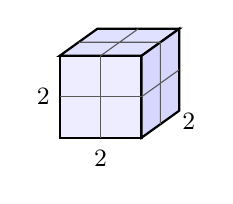
\begin{tikzpicture}[scale=0.52,x={(1cm,0cm)},y={(0.46cm,0.33cm)},z={(0cm,1cm)}]
  \draw[thick,fill=blue!7]  (0,0,0)--(2,0,0)--(2,0,2)--(0,0,2)--cycle;
  \draw[thick,fill=blue!12] (0,0,2)--(2,0,2)--(2,2,2)--(0,2,2)--cycle;
  \draw[thick,fill=blue!16] (2,0,0)--(2,2,0)--(2,2,2)--(2,0,2)--cycle;
  \draw[gray!70!black] (1,0,0)--(1,0,2) (0,0,1)--(2,0,1);
  \draw[gray!70!black] (1,0,2)--(1,2,2) (0,1,2)--(2,1,2);
  \draw[gray!70!black] (2,1,0)--(2,1,2) (2,0,1)--(2,2,1);
  \node[font=\small] at (1,0,-0.5) {$2$};
  \node[font=\small] at (-0.4,0,1) {$2$};
  \node[font=\small] at (2.6,1.2,0) {$2$};
\end{tikzpicture}}

% ----------------------------------------------------------------
% The shapes of the first four dimensions, each drawn with a dot on
% every corner so that the corners can be counted from the picture.
% The dot radius is given in points, so it stays the same size however
% the picture is scaled.
\newcommand{\pointpic}[2]{%
\begin{tikzpicture}[scale=#1]
  \fill[blue!45!black] (0,0) circle (#2);
\end{tikzpicture}}
\newcommand{\linepic}[2]{%
\begin{tikzpicture}[scale=#1]
  \draw[blue!45!black,thick] (0,0)--(2,0);
  \fill[blue!45!black] (0,0) circle (#2) (2,0) circle (#2);
\end{tikzpicture}}
\newcommand{\squarecorners}[2]{%
\begin{tikzpicture}[scale=#1]
  \draw[blue!45!black,thick] (0,0) rectangle (2,2);
  \foreach \a in {0,2} \foreach \b in {0,2} \fill[blue!45!black] (\a,\b) circle (#2);
\end{tikzpicture}}
\newcommand{\cubecorners}[2]{%
\begin{tikzpicture}[scale=#1,x={(1cm,0cm)},y={(0.5cm,0.36cm)},z={(0cm,1cm)},
    line join=round]
  \draw[blue!45!black,thick] (0,0,0)--(2,0,0)--(2,2,0)--(0,2,0)--cycle;
  \draw[blue!45!black,thick] (0,0,2)--(2,0,2)--(2,2,2)--(0,2,2)--cycle;
  \draw[blue!45!black,thick] (0,0,0)--(0,0,2) (2,0,0)--(2,0,2)
    (2,2,0)--(2,2,2) (0,2,0)--(0,2,2);
  \foreach \a in {0,2} \foreach \b in {0,2} \foreach \c in {0,2}
    \fill[blue!45!black] (\a,\b,\c) circle (#2);
\end{tikzpicture}}

% A tesseract, drawn the way a cube is drawn on paper: a small cube
% inside a large cube, with every corner of one joined to the matching
% corner of the other. In four dimensions all eight cubes in the
% picture are the same size and all the joining lines are the same
% length, so the picture stretches the shape in the same way that a
% drawing of a cube stretches its square faces.
\newcommand{\tesspic}[2]{%
\begin{tikzpicture}[scale=#1,x={(1cm,0cm)},y={(0.5cm,0.36cm)},z={(0cm,1cm)},
    line join=round]
  \foreach \a in {0,4} \foreach \b in {0,4} \foreach \c in {0,4}
    \draw[gray!55] (\a,\b,\c) -- ({1+\a/2},{1+\b/2},{1+\c/2});
  \draw[orange!65!black,thick] (1,1,1)--(3,1,1)--(3,3,1)--(1,3,1)--cycle;
  \draw[orange!65!black,thick] (1,1,3)--(3,1,3)--(3,3,3)--(1,3,3)--cycle;
  \draw[orange!65!black,thick] (1,1,1)--(1,1,3) (3,1,1)--(3,1,3)
    (3,3,1)--(3,3,3) (1,3,1)--(1,3,3);
  \draw[blue!45!black,thick] (0,0,0)--(4,0,0)--(4,4,0)--(0,4,0)--cycle;
  \draw[blue!45!black,thick] (0,0,4)--(4,0,4)--(4,4,4)--(0,4,4)--cycle;
  \draw[blue!45!black,thick] (0,0,0)--(0,0,4) (4,0,0)--(4,0,4)
    (4,4,0)--(4,4,4) (0,4,0)--(0,4,4);
  \foreach \a in {0,4} \foreach \b in {0,4} \foreach \c in {0,4} {%
    \fill[blue!45!black] (\a,\b,\c) circle (#2);
    \fill[orange!65!black] ({1+\a/2},{1+\b/2},{1+\c/2}) circle (#2);}
\end{tikzpicture}}

% Characters this language's font has not got are borrowed from another,
% rather than being silently dropped - see docs/translated-sheet-latex.md
\directlua{%
  if luaotfload and luaotfload.add_fallback then
    luaotfload.add_fallback("eallatinfallback",
      { "Noto Serif:mode=harf;" })
  else
    tex.error("this luaotfload is too old to register a fallback font")
  end
}
\usepackage[english]{babel}
\babelprovide[import]{polish}
\babelfont[polish]{rm}[Renderer=Harfbuzz, BoldFont={Noto Serif}, ItalicFont={Noto Serif}, BoldItalicFont={Noto Serif}, RawFeature={fallback=eallatinfallback}]{Noto Serif}
\babelfont[polish]{sf}[Renderer=Harfbuzz, BoldFont={Noto Serif}, ItalicFont={Noto Serif}, BoldItalicFont={Noto Serif}, RawFeature={fallback=eallatinfallback}]{Noto Serif}
\newcommand{\ealtext}[1]{\foreignlanguage{polish}{#1}}
\newcommand{\ealtextblock}[1]{{\raggedright\foreignlanguage{polish}{#1}\par}}
% ================================================================
% EAL layout helpers
% ================================================================
\usepackage{xcolor}

\definecolor{ealkeycolour}{RGB}{0,128,0}
\definecolor{ealenglish}{RGB}{0,0,0}
\definecolor{ealtwocolour}{RGB}{112,48,160}

\newsavebox{\ealboxen}
\newsavebox{\ealboxtr}
\newlength{\ealglosswd}
\newlength{\ealglossraise}
\setlength{\ealglossraise}{1.15em}

% a tier 3 word, in English and in translation alike
\newcommand{\ealkey}[1]{\textcolor{ealkeycolour}{#1}}
\newcommand{\ealkeytr}[1]{\textcolor{ealkeycolour}{\ealtext{#1}}}

% One translated word above one English word. Built from kernel
% primitives, never a tabular, which would break wherever the sheet
% loads array, booktabs or tabularx. The box is as wide as the wider of
% the two, so a long translation pushes its neighbours aside instead of
% overlapping them, and it claims its full height so a table row or a
% TikZ node makes room for it.
\newcommand{\ealgloss}[2]{%
  \sbox{\ealboxen}{\ealkey{#1}}%
  \sbox{\ealboxtr}{\small\textcolor{ealtwocolour}{\ealtext{#2}}}%
  \setlength{\ealglosswd}{\wd\ealboxen}%
  \ifdim\wd\ealboxtr>\ealglosswd\setlength{\ealglosswd}{\wd\ealboxtr}\fi
  \leavevmode
  \makebox[\ealglosswd][c]{%
    \makebox[0pt][c]{\usebox{\ealboxen}}%
    \makebox[0pt][c]{\raisebox{\ealglossraise}{\usebox{\ealboxtr}}}%
  }%
}

% opens up line spacing around a block of glosses, so the raised
% translations sit clear of the line above
\newenvironment{ealglossed}{\par\linespread{2.1}\selectfont\ignorespaces}{\par}

% a whole translated sentence above its English counterpart. block level,
% so it does not belong inside a tabular cell
\newcommand{\ealpara}[2]{%
  \par\addvspace{0.5\baselineskip}%
  {\color{ealtwocolour}\ealtextblock{#1}}%
  \penalty200
  {\color{ealenglish}#2\par}%
  \addvspace{0.5\baselineskip}%
}

\begin{document}
\begin{ealglossed}

\begin{center}
  {\Large\bfseries \ealgloss{Indices}{wykładnik} and \ealgloss{Roots}{pierwiastek}}\\[2pt]
\end{center}

\begin{keyidea}
An \textbf{\ealgloss{index}{wykładnik}} tells us how many times a number is multiplied by itself. So $5^3$ means $5\times5\times5$. The plural
of \ealgloss{index}{wykładnik} is \textbf{\ealgloss{indices}{wykładnik}}. A \ealgloss{root}{pierwiastek} undoes an \ealgloss{index}{wykładnik}.
\end{keyidea}

\parttitle{1}{\ealgloss{Indices}{wykładnik} and \ealgloss{roots}{pierwiastek} of numbers}

\begin{minipage}[t]{0.56\linewidth}
\vspace{0pt}
$3^2$ is read ``three \ealgloss{squared}{podnieść do kwadratu; kwadrat}''. $2^3$ is read ``two \ealgloss{cubed}{sześcian}''. 

\vspace{4pt}
The \textbf{\ealgloss{square root}{pierwiastek}} of a number is the value that gives that number when it (the square root) is
multiplied by itself, so $\sqrt{9}=3$. The \textbf{\ealgloss{cube root}{pierwiastek sześcienny}} of a number is
the value that gives that number when three of them are multiplied together, so
\mbox{$\sqrt[3]{8}=2$}.
\end{minipage}\hfill
\begin{minipage}[t]{0.41\linewidth}
\vspace{0pt}
\centering
\begin{tabular}{@{}c@{\hspace{0.9em}}c@{}}
\squarepic & \cubepic\\[4pt]
{\small $3^2=3\times3=9$} & {\small $2^3=2\times2\times2=8$}\\
\end{tabular}
\end{minipage}

\vspace{2pt}
\begin{notation}{\ealgloss{indices}{wykładnik} and \ealgloss{roots}{pierwiastek}}
\renewcommand{\arraystretch}{2.2}%
\begin{tabular}{@{}>{\large}p{4.3cm}@{\hspace{0.8em}}p{5.0cm}@{\hspace{0.8em}}l@{}}
$a^2=a\times a$ & ``$a$ \ealgloss{squared}{podnieść do kwadratu; kwadrat}'' & for example \; $7^2=7\times7=49$\\
$a^3=a\times a\times a$ & ``$a$ \ealgloss{cubed}{sześcian}'' & for example \; $2^3=2\times2\times2=8$\\
$\sqrt{a}$ & the \ealgloss{square root}{pierwiastek} of $a$ & for example \; $\sqrt{49}=7$\\
$\sqrt[3]{a}$ & the \ealgloss{cube root}{pierwiastek sześcienny} of $a$ & for example \; $\sqrt[3]{8}=2$\\
\end{tabular}

\vspace{2pt}
An \ealgloss{index}{wykładnik} multiplies the \ealgloss{base}{podstawa} by itself, and a \ealgloss{root}{pierwiastek} finds the \ealgloss{base}{podstawa}
again.
\end{notation}

\begin{enumerate}

\item Work out each calculation on the left and draw a line joining it to
its answer on the right. Check your answers on a calculator afterwards.
\matchup{{$5^2$},{$\sqrt{100}$},{$2^3$},{$0.2^2$},{$\sqrt{0.25}$},{$10^3$},
  {$\sqrt[3]{8}$},{$1.5^2$}}%
  {{$0.5$},{$8$},{$2$},{$25$},{$1000$},{$0.04$},{$2.25$},{$10$}}

\end{enumerate}

\begin{enumerate}[resume]

\newpage{}

\item The shapes are not drawn to \ealgloss{scale}{skalować}.


\begin{enumerate}
  \item A square patio has sides of length $6$ m. Work out its \ealgloss{area}{pole}.

\vspace{2pt}
\begin{minipage}[t]{0.34\linewidth}
\centering
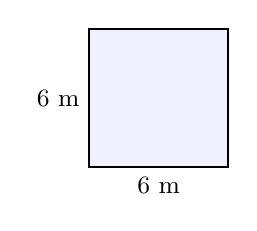
\begin{tikzpicture}[baseline=(current bounding box.north),scale=0.8]
  \draw[thick,fill=blue!6] (0,0) rectangle (2.2,2.2);
  \node[below,font=\small] at (1.1,0) {$6$ m};
  \node[left,font=\small] at (0,1.1) {$6$ m};
\end{tikzpicture}
\end{minipage}%
\begin{minipage}[t]{0.62\linewidth}
\vspace{1.4em}
\ealgloss{Area}{pole} $=6^2=6\times6=\ansline[1.8cm]$ m$^2$
\end{minipage}

  \item A second square patio has an \ealgloss{area}{pole} of $144$ m$^2$. Work out the length
        of one of its sides.

\vspace{2pt}
\begin{minipage}[t]{0.34\linewidth}
\centering
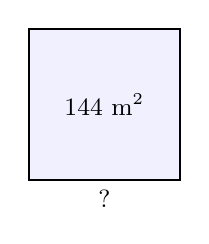
\begin{tikzpicture}[baseline=(current bounding box.north),scale=0.8]
  \draw[thick,fill=blue!6] (0,0) rectangle (2.4,2.4);
  \node[font=\small] at (1.2,1.2) {$144$ m$^2$};
  \node[below,font=\small] at (1.2,0) {$?$};
\end{tikzpicture}
\end{minipage}%
\begin{minipage}[t]{0.62\linewidth}
\vspace{1.4em}
Side $=\sqrt{144}=\ansline[1.8cm]$ m
\end{minipage}

  \item A storage box is a \ealgloss{cube}{sześcian} with \ealgloss{edges}{krawędź} of length $4$ cm. Work out its
        \ealgloss{volume}{objętość}.

\vspace{2pt}
\begin{minipage}[t]{0.34\linewidth}
\centering
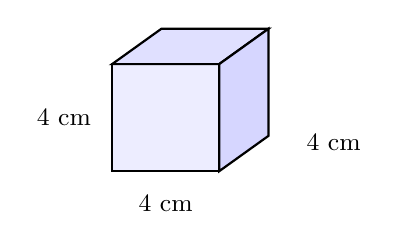
\begin{tikzpicture}[baseline=(current bounding box.north),scale=0.68,
    x={(1cm,0cm)},y={(0.46cm,0.33cm)},z={(0cm,1cm)}]
  \draw[thick,fill=blue!7]  (0,0,0)--(2,0,0)--(2,0,2)--(0,0,2)--cycle;
  \draw[thick,fill=blue!12] (0,0,2)--(2,0,2)--(2,2,2)--(0,2,2)--cycle;
  \draw[thick,fill=blue!16] (2,0,0)--(2,2,0)--(2,2,2)--(2,0,2)--cycle;
  \node[font=\small] at (1,0,-0.6) {$4$ cm};
  \node[font=\small] at (-0.9,0,1) {$4$ cm};
  \node[font=\small] at (3.4,1.6,0) {$4$ cm};
\end{tikzpicture}
\end{minipage}%
\begin{minipage}[t]{0.62\linewidth}
\vspace{1.4em}
\ealgloss{Volume}{objętość} $=4^3=\ansline[3.4cm]$ cm$^3$
\end{minipage}

  \item A second storage box is a \ealgloss{cube}{sześcian} with a \ealgloss{volume}{objętość} of $125$ cm$^3$. Work out
        the length of one of its \ealgloss{edges}{krawędź}.

\vspace{2pt}
\begin{minipage}[t]{0.34\linewidth}
\centering
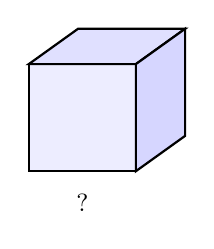
\begin{tikzpicture}[baseline=(current bounding box.north),scale=0.68,
    x={(1cm,0cm)},y={(0.46cm,0.33cm)},z={(0cm,1cm)}]
  \draw[thick,fill=blue!7]  (0,0,0)--(2,0,0)--(2,0,2)--(0,0,2)--cycle;
  \draw[thick,fill=blue!12] (0,0,2)--(2,0,2)--(2,2,2)--(0,2,2)--cycle;
  \draw[thick,fill=blue!16] (2,0,0)--(2,2,0)--(2,2,2)--(2,0,2)--cycle;
  \node[font=\small] at (1,0,-0.6) {$?$};
\end{tikzpicture}

\vspace{1pt}
{\small \ealgloss{Volume}{objętość} $=125$ cm$^3$}
\end{minipage}%
\begin{minipage}[t]{0.62\linewidth}
\vspace{1.4em}
\ealgloss{Edge}{krawędź} $=\ansline[3.4cm]$ cm
\end{minipage}

  \item A square floor tile has an \ealgloss{area}{pole} of $0.25$ m$^2$. Work out the length of
        one of its sides.

\vspace{2pt}
\begin{minipage}[t]{0.34\linewidth}
\centering
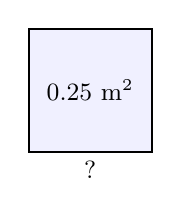
\begin{tikzpicture}[baseline=(current bounding box.north),scale=0.8]
  \draw[thick,fill=blue!6] (0,0) rectangle (1.95,1.95);
  \node[font=\small] at (0.975,0.975) {$0.25$ m$^2$};
  \node[below,font=\small] at (0.975,0) {$?$};
\end{tikzpicture}
\end{minipage}%
\begin{minipage}[t]{0.62\linewidth}
\vspace{1.4em}
Side $=\sqrt{0.25}=\ansline[1.8cm]$ m
\end{minipage}

  \item A square garden has an \ealgloss{area}{pole} of $50$ m$^2$. Without a calculator, find
        the two \ealgloss{whole numbers}{liczba całkowita nieujemna} that the length of one side lies between. Explain
        how you know.

\vspace{2pt}
\begin{minipage}[t]{0.34\linewidth}
\centering
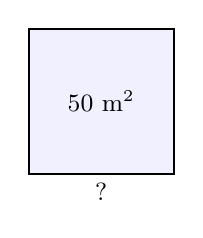
\begin{tikzpicture}[baseline=(current bounding box.north),scale=0.8]
  \draw[thick,fill=blue!6] (0,0) rectangle (2.3,2.3);
  \node[font=\small] at (1.15,1.15) {$50$ m$^2$};
  \node[below,font=\small] at (1.15,0) {$?$};
\end{tikzpicture}
\end{minipage}%
\begin{minipage}[t]{0.62\linewidth}
\vspace{1.4em}
The side is between \ansline[1.2cm] m and \ansline[1.2cm] m, because

\vspace{14pt}
\ansline[9.5cm]
\end{minipage}
\end{enumerate}

\end{enumerate}

\vspace{6pt}

\newpage{}

\parttitle{2}{\ealgloss{Indices}{wykładnik} and \ealgloss{algebraic variables}{zmienna algebraiczna}}

An \textbf{\ealgloss{algebraic variable}{zmienna algebraiczna}}, such as $a$, $x$ or $m$, could be any number. Just like $5^3=5\times5\times5$, $a^3$ means $a\times a\times a$.


\begin{warning}
In $5a^2$ the \ealgloss{index}{wykładnik} belongs to the $a$ only, so $5a^2=5\times a\times a$. It is
\textbf{not} $5a\times5a$. If $a=2$ then $5a^2=5\times2\times2=20$, but
$5a\times5a=10\times10=100$.
\end{warning}

\begin{wex}{writing a \ealgloss{fraction}{ułamek} in \ealgloss{index form}{postać potęgowa}}
\small
Write $\dfrac{a\times a\times a}{b\times b}$ in \ealgloss{index form}{postać potęgowa}.

\smallskip
\renewcommand{\arraystretch}{2.4}
\begin{tabular}{@{}l@{\hspace{1.2em}}l@{}}
\textbf{Step 1 --- count the \ealgloss{numerator}{licznik}.}
  & $a$ appears $3$ times, so the \ealgloss{numerator}{licznik} is $a^3$.\\
\textbf{Step 2 --- count the \ealgloss{denominator}{mianownik}.}
  & $b$ appears $2$ times, so the \ealgloss{denominator}{mianownik} is $b^2$.\\
\textbf{Step 3 --- write the \ealgloss{fraction}{ułamek}.}
  & $\dfrac{a\times a\times a}{b\times b}=\dfrac{a^3}{b^2}$\\
\end{tabular}
\end{wex}


\begin{enumerate}[resume]

\item Write each \ealgloss{expression}{wyrażenie} in \ealgloss{index form}{postać potęgowa}. Fill in the gaps in parts (a) and
(b), then \ealgloss{simplify}{uprościć} the remaining \ealgloss{expressions}{wyrażenie} in the same way.
\begin{enumerate}
  \item $a\times a\times a\times a=a^{\boxgap}$
  \item $\dfrac{c\times c\times c}{d\times d}=\dfrac{c^{\boxgap[7pt]}}{d^{\boxgap[7pt]}}$
\end{enumerate}
\vspace{4pt}
\begin{multicols}{3}
\begin{enumerate}[resume]
  \item $b\times b\times b\times b\times b$
  \item $3\times m\times m$
  \item $\dfrac{p\times p\times p}{q\times q\times q\times q}$
  \item $\dfrac{2\times x\times x\times x}{y\times y}$
  \item $\dfrac{a\times a\times b\times b\times b}{c\times c}$
  \item $\dfrac{t\times t}{5\times u\times u\times u}$
\end{enumerate}
\end{multicols}
\vspace{8em}

\item Write each \ealgloss{expression}{wyrażenie} out in full as a multiplication. The first one is
done for you.
\begin{enumerate}
  \item $x^3=x\times x\times x$
\end{enumerate}
\vspace{2pt}
\begin{multicols}{2}
\begin{enumerate}[resume]
  \item $y^5=\ansline[4cm]$
  \item $4t^2=\ansline[4cm]$
  \item $\dfrac{m^2}{n^3}=\ansline[4cm]$
  \item $\dfrac{a^4}{b}=\ansline[4cm]$
\end{enumerate}
\end{multicols}

\end{enumerate}

\vspace{6pt}

\newpage{}

\parttitle{3}{\ealgloss{Cancelling}{skracanie} \ealgloss{factors}{dzielnik} in a \ealgloss{fraction}{ułamek}}

A \ealgloss{fraction}{ułamek} stays the same
value when the \ealgloss{numerator}{licznik} and the \ealgloss{denominator}{mianownik} are both divided by the same
number. Since the new \ealgloss{fraction}{ułamek} is \textbf{\ealgloss{equivalent}{równoważny}} to the original.

\begin{keyidea}
When the \ealgloss{numerator}{licznik} and the \ealgloss{denominator}{mianownik} are written as multiplications, a \ealgloss{factor}{dzielnik}
that appears in both can be divided out of both. This is called
\textbf{\ealgloss{cancelling}{skracanie}}, and it is written by crossing the \ealgloss{factor}{dzielnik} out on the top
and on the bottom.
\end{keyidea}

\begin{wex}{\ealgloss{simplify}{uprościć} $\dfrac{12}{18}$}
\small
\renewcommand{\arraystretch}{2.6}
\begin{tabular}{@{}l@{\hspace{1.2em}}l@{}}
\textbf{Step 1 --- write the \ealgloss{numerator}{licznik} and the \ealgloss{denominator}{mianownik} as multiplications.}
  & $\dfrac{12}{18}=\dfrac{2\times2\times3}{2\times3\times3}$\\
\textbf{Step 2 --- cross out each \ealgloss{factor}{dzielnik} that appears in both.}
  & $\dfrac{12}{18}=\dfrac{\cancel{2}\times2\times\cancel{3}}
    {\cancel{2}\times\cancel{3}\times3}$\\
\textbf{Step 3 --- multiply what is left on the top and on the bottom.}
  & $\dfrac{12}{18}=\dfrac{2}{3}$\\
\end{tabular}
\end{wex}

\begin{enumerate}[resume]

\item \ealgloss{Simplify}{uprościć} each \ealgloss{fraction}{ułamek} by \ealgloss{cancelling}{skracanie}. Fill in the gaps in parts (a) and
(b), then do parts (c) to (f) in the same way.
\begin{enumerate}
  \item $\dfrac{8}{12}=\dfrac{2\times2\times2}{2\times2\times3}
         =\dfrac{\cancel{2}\times\cancel{2}\times2}
          {\cancel{2}\times\cancel{2}\times3}
         =\dfrac{\boxgap[11pt]}{\boxgap[11pt]}$
  \item $\dfrac{15}{25}=\dfrac{5\times3}{5\times\boxgap[11pt]}
         =\dfrac{\boxgap[11pt]}{\boxgap[11pt]}$
\end{enumerate}
\vspace{6pt}
\begin{multicols}{4}
\begin{enumerate}[resume]
  \item $\dfrac{18}{24}$
  \item $\dfrac{14}{21}$
  \item $\dfrac{45}{60}$
  \item $\dfrac{24}{36}$
\end{enumerate}
\end{multicols}
\vspace{6em}

% The list inside multicols does not pass its count on, so the letters
% after (f) are started by hand.
\begin{enumerate}[start=7]
  \item $12$ of the $28$ pupils in a class walk to school. The picture shows
        the class, with the pupils who walk shaded. Write the \ealgloss{fraction}{ułamek} of the
        class who walk to school in its \ealgloss{simplest form}{najprostsza postać}.

\vspace{4pt}
\begin{minipage}[t]{0.40\linewidth}
\centering
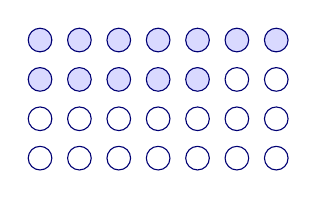
\begin{tikzpicture}[baseline=(current bounding box.north),scale=0.5]
  \foreach \i in {0,...,27} {
    \pgfmathtruncatemacro{\col}{mod(\i,7)}
    \pgfmathtruncatemacro{\row}{\i/7}
    \ifnum\i<12
      \draw[blue!45!black,fill=blue!15] (\col,-\row) circle (0.3);
    \else
      \draw[blue!45!black,fill=white] (\col,-\row) circle (0.3);
    \fi}
\end{tikzpicture}
\end{minipage}%
\begin{minipage}[t]{0.56\linewidth}
\vspace{1.2em}
\ealgloss{Fraction}{ułamek} who walk $=\dfrac{12}{28}=\ansline[3cm]$
\end{minipage}

\vspace{3em}
  \item A cake mixture weighs $120$ g, and $45$ g of it is sugar. Write the
        \ealgloss{fraction}{ułamek} of the mixture that is sugar in its \ealgloss{simplest form}{najprostsza postać}.

\vspace{5em}
\end{enumerate}

\end{enumerate}


\newpage{}

\ealgloss{Algebraic variables}{zmienna algebraiczna} \ealgloss{cancel}{skracanie} in the same way as numbers. When every \ealgloss{factor}{dzielnik} on the bottom \ealgloss{cancels}{skracanie}, the \ealgloss{denominator}{mianownik}
is $1$, not nothing, a \ealgloss{fraction}{ułamek} with a \ealgloss{denominator}{mianownik} of $1$ is equal to its
\ealgloss{numerator}{licznik}.

\begin{wex}{\ealgloss{cancelling}{skracanie} with numbers and variables}
\small
\renewcommand{\arraystretch}{2.6}
\begin{tabular}{@{}l@{\hspace{1.5em}}l@{}}
$\dfrac{a\times a\times a}{a\times a}
  =\dfrac{\cancel{a}\times\cancel{a}\times a}{\cancel{a}\times\cancel{a}}
  =\dfrac{a}{1}=a$
  & every \ealgloss{factor}{dzielnik} on the bottom \ealgloss{cancels}{skracanie}, leaving $1$\\
$\dfrac{2\times3\times a\times a}{2\times a}
  =\dfrac{\cancel{2}\times3\times\cancel{a}\times a}
   {\cancel{2}\times\cancel{a}}=\dfrac{3\times a}{1}=3a$
  & the numbers and the variables are \ealgloss{cancelled}{skracanie} separately\\
\end{tabular}
\end{wex}

\begin{enumerate}[resume]

\item \ealgloss{Simplify}{uprościć} each \ealgloss{fraction}{ułamek} by \ealgloss{cancelling}{skracanie}, then write the answer in \ealgloss{index form}{postać potęgowa}. Fill in the gaps in part (a) first.
\begin{enumerate}
  \item $\dfrac{a\times a\times a\times a}{a\times a}
         =\dfrac{\cancel{a}\times\cancel{a}\times a\times a}
          {\cancel{a}\times\cancel{a}}=\dfrac{a\times a}{1}=a^{\boxgap}$
\end{enumerate}
\vspace{6pt}
\begin{enumerate}[resume]
  \item $\dfrac{b\times b\times b\times b\times b}{b\times b} =$
  \item $\dfrac{2\times2\times m\times m}{2\times m}=$
  \item $\dfrac{3\times5\times p\times p\times p}{5\times p}=$
  \item $\dfrac{x\times x\times y}{x\times y\times y}=$
  \item $\dfrac{2\times3\times t\times t}{3\times3\times t}=$
  \item $\dfrac{4\times x\times x\times y}{6\times x\times y\times y}=$
  \item $\dfrac{5\times5\times a\times b\times b}{5\times a\times a\times b}=$
  \item Lena \ealgloss{simplifies}{uprościć} $\dfrac{a\times a}{a\times a\times a}$ and writes $a$.
        Explain the mistake Lena has made, and write down the correct answer.

\vspace{6pt}
\ansline[16cm]

\vspace{16pt}
\ansline[16cm]
\end{enumerate}
\vspace{10em}

\end{enumerate}

\newpage{}

\parttitle{4}{\ealgloss{Simplifying}{uprościć} \ealgloss{fractions}{ułamek} written with \ealgloss{indices}{wykładnik}}

A \ealgloss{fraction}{ułamek} written with \ealgloss{indices}{wykładnik} is \ealgloss{simplified}{uprościć} in the same way. We write each
\ealgloss{power}{potęga} out in full as a multiplication, \ealgloss{cancel}{skracanie} the \ealgloss{factors}{dzielnik} that appear on the
top and on the bottom, and write what is left in \ealgloss{index form}{postać potęgowa}.

\begin{wex}{\ealgloss{simplifying}{uprościć} \ealgloss{fractions}{ułamek} written with \ealgloss{indices}{wykładnik}}
\small
\renewcommand{\arraystretch}{2.6}
\begin{tabular}{@{}l@{\hspace{2em}}l@{}}
$\dfrac{a^5}{a^2}
  =\dfrac{\cancel{a}\times\cancel{a}\times a\times a\times a}
   {\cancel{a}\times\cancel{a}}=a^3$
  & two of the five $a$s \ealgloss{cancel}{skracanie}, leaving three\\
$\dfrac{6a^3}{2a}
  =\dfrac{\cancel{2}\times3\times\cancel{a}\times a\times a}
   {\cancel{2}\times\cancel{a}}=3a^2$
  & $6=2\times3$, so a \ealgloss{factor}{dzielnik} of $2$ \ealgloss{cancels}{skracanie} as well\\
\end{tabular}
\end{wex}

\begin{enumerate}[resume]

\item \ealgloss{Simplify}{uprościć} each \ealgloss{fraction}{ułamek} on the left. Draw a line joining it to its answer
on the right.

\vspace{4pt}
\matchup[1.6]{{$\dfrac{a^5}{a^2}$},{$\dfrac{a^2}{a^2}$},{$\dfrac{6a^4}{2a^2}$},
  {$\dfrac{a^3b}{ab}$},{$\dfrac{4a^2}{8a}$},{$\dfrac{a^2b^3}{a^2b}$},
  {$\dfrac{10a^3}{5a^3}$},{$\dfrac{a^6}{a^2}$}}%
  {{$b^2$},{$a^4$},{$2$},{$a^3$},{$\dfrac{a}{2}$},{$1$},{$a^2$},{$3a^2$}}

\end{enumerate}

\newpage

\begin{enumerate}[resume]

\item
\begin{enumerate}
  \item Write down three different \ealgloss{fractions}{ułamek} that \ealgloss{simplify}{uprościć} to $2a^2$. One of
        them must have a number other than $1$ in the \ealgloss{denominator}{mianownik}.

\vspace{12pt}
\ansline[3.4cm]\hfill \ansline[3.4cm]\hfill \ansline[3.4cm]

\vspace{12pt}
  \item Write down a \ealgloss{fraction}{ułamek} (not equal to $\frac{a^2}{b}$) using the variables $a$ and $b$ that \ealgloss{simplifies}{uprościć}
        to $\frac{a^2}{b}$.

\vspace{16pt}
\ansline[5cm]


\vspace{8pt}
\item Write down a \ealgloss{fraction}{ułamek} using the variables $x$, $y$ and $z$ that \ealgloss{simplifies}{uprościć} to
      $\frac{1}{xy^2}$.

\vspace{16pt}
\ansline[5cm]


\vspace{8pt}
  \item Ben says that $\frac{3a^2}{3a^2}=0$, because every \ealgloss{factor}{dzielnik} on the top
        and on the bottom \ealgloss{cancels}{skracanie} and nothing is left. Explain the mistake Ben
        has made, and write down the correct answer.

\vspace{6pt}
\ansline[16cm]

\vspace{16pt}
\ansline[16cm]
\end{enumerate}

\item In this question we find a quicker way to \ealgloss{simplify}{uprościć} a \ealgloss{fraction}{ułamek} such as
$\dfrac{a^7}{a^3}$.
\begin{enumerate}
  \item \ealgloss{Simplify}{uprościć} each \ealgloss{fraction}{ułamek} by writing it out in full and \ealgloss{cancelling}{skracanie}. Give
        each answer in \ealgloss{index form}{postać potęgowa}.

\vspace{8pt}
$\dfrac{a^7}{a^3}=\ansline[2.4cm]$ \hfill $\dfrac{b^9}{b^4}=\ansline[2.4cm]$
\hfill $\dfrac{c^6}{c^5}=\ansline[2.4cm]$

\vspace{3.5em}
  \item Look at the \ealgloss{indices}{wykładnik} in each \ealgloss{fraction}{ułamek} and in its answer. Describe a
        quicker way to find the answer without writing the powers out in full.

\vspace{6pt}
\ansline[16cm]

\vspace{16pt}
\ansline[16cm]

\vspace{6pt}
  \item Use your quicker way to \ealgloss{simplify}{uprościć} these \ealgloss{fractions}{ułamek}.

\vspace{8pt}
$\dfrac{x^{20}}{x^{13}}=\ansline[2.4cm]$ \hspace{3em}
$\dfrac{y^{100}}{y^{99}}=\ansline[2.4cm]$

\vspace{6pt}
  \item Use your quicker way on $\dfrac{a^3}{a^3}$. \ealgloss{Cancelling}{skracanie} shows that
        $\dfrac{a^3}{a^3}=1$. What does this suggest $a^0$ is equal to?

\vspace{10pt}
$\dfrac{a^3}{a^3}=a^{\boxgap}$ \hspace{3em} so \hspace{3em} $a^0=\ansline[2.4cm]$
\end{enumerate}

\end{enumerate}

\newpage{}

\vspace{6pt}

\parttitle{5}{Extension: \ealgloss{factorials}{silnia}, \ealgloss{negative}{ujemny} numbers and the fourth \ealgloss{dimension}{wymiar}}

The \textbf{\ealgloss{factorial}{silnia}} of a \ealgloss{whole number}{liczba całkowita nieujemna} is written with an exclamation mark
after it. The \ealgloss{expression}{wyrażenie} $n!$ means multiply together every \ealgloss{whole number}{liczba całkowita nieujemna} from
$n$ down to $1$, so $5!=5\times4\times3\times2\times1=120$.

$10!=10\times9\times8\times7\times6\times5\times4\times3\times2\times1=3\,628\,800$.

\begin{enumerate}[resume]

\item Work out each \ealgloss{factorial}{silnia}.
\begin{multicols}{4}
\begin{enumerate}
  \item $3!=\ansline[1.8cm]$
  \item $4!=\ansline[1.8cm]$
  \item $6!=\ansline[1.8cm]$
  \item $1!=\ansline[1.8cm]$
\end{enumerate}
\end{multicols}

\end{enumerate}

\begin{wex}{\ealgloss{simplify}{uprościć} $\dfrac{6!}{4!}$}
\small
Both \ealgloss{factorials}{silnia} are written out in full. Every \ealgloss{whole number}{liczba całkowita nieujemna} from $4$ downwards
appears on the top and on the bottom, so all of those \ealgloss{factors}{dzielnik} \ealgloss{cancel}{skracanie}.

\smallskip
\[\frac{6!}{4!}
  =\frac{6\times5\times\cancel{4}\times\cancel{3}\times\cancel{2}\times\cancel{1}}
   {\cancel{4}\times\cancel{3}\times\cancel{2}\times\cancel{1}}
  =6\times5=30\]
\end{wex}

\begin{enumerate}[resume]

\item \ealgloss{Simplify}{uprościć} each \ealgloss{expression}{wyrażenie} by writing the \ealgloss{factorials}{silnia} out in full and
\ealgloss{cancelling}{skracanie}. Do not work the \ealgloss{factorials}{silnia} out first.
\begin{multicols}{3}
\begin{enumerate}
  \item $\dfrac{5!}{3!}$
  \item $\dfrac{10!}{9!}$
  \item $\dfrac{8!}{6!}$
  \item $\dfrac{7!}{5!\times2!}$
  \item $\dfrac{100!}{98!}$
  \item $\dfrac{12!}{10!\times2!}$
\end{enumerate}
\end{multicols}
\vspace{9em}

\item For any \ealgloss{whole number}{liczba całkowita nieujemna} $n$ that is greater than $1$, the \ealgloss{expression}{wyrażenie}
$\dfrac{n!}{(n-1)!}$ always \ealgloss{simplifies}{uprościć} to $n$. Explain why.

\vspace{6pt}
\ansline[16cm]

\vspace{16pt}
\ansline[16cm]

\vspace{16pt}
\ansline[16cm]

\newpage{}

\item When the \ealgloss{base}{podstawa} is \ealgloss{negative}{ujemny}, the brackets show that the whole \ealgloss{negative}{ujemny}
number is multiplied by itself, so $(-2)^3=(-2)\times(-2)\times(-2)$.
\begin{enumerate}
  \item Complete the table.

\vspace{2pt}
\begin{center}
\renewcommand{\arraystretch}{2.4}
\begin{tabular}{|>{\centering\arraybackslash}p{2.4cm}|>{\centering\arraybackslash}p{6.4cm}|>{\centering\arraybackslash}p{2.4cm}|}
\hline
\textbf{\ealgloss{Expression}{wyrażenie}} & \textbf{Written out in full} & \textbf{Answer}\\
\hline
$(-2)^2$ & $(-2)\times(-2)$ & $4$\\ \hline
$(-2)^3$ & $(-2)\times(-2)\times(-2)$ & \\ \hline
$(-2)^4$ & & \\ \hline
$(-3)^2$ & & \\ \hline
$(-3)^3$ & & \\ \hline
\end{tabular}
\end{center}

  \item Write down what you notice about the \ealgloss{sign}{znak} of the answer when the \ealgloss{index}{wykładnik}
        is \ealgloss{even}{parzysty}, and when the \ealgloss{index}{wykładnik} is \ealgloss{odd}{liczba nieparzysta}.

\vspace{6pt}
\ansline[16cm]

\vspace{16pt}
  \item Explain why this happens.

\vspace{6pt}
\ansline[16cm]
\end{enumerate}

\end{enumerate}


\begin{enumerate}[resume]

\item
\begin{enumerate}
  \item Work out $3\times3$ and $(-3)\times(-3)$. Write down both of the
        numbers that give $9$ when they are multiplied by themselves.

\vspace{8pt}
\ansline[5.5cm] \hspace{1.5em} and \hspace{1.5em} \ansline[5.5cm]

\vspace{6pt}
The symbol $\sqrt{\phantom{a}}$ means the \ealgloss{positive}{liczba dodatnia} \ealgloss{square root}{pierwiastek} only, so
$\sqrt{9}=3$.

\vspace{6pt}
  \item Work out $\sqrt{-9}$ on your calculator. Write down what the calculator
        shows, and explain why.

\vspace{6pt}
\ansline[16cm]

\vspace{16pt}
\ansline[16cm]

\vspace{6pt}
  \item Work out $(-2)\times(-2)\times(-2)$. Use your answer to write down
        $\sqrt[3]{-8}$.

\vspace{8pt}
\ansline[5.5cm] \hspace{1.5em} so \hspace{1.5em} $\sqrt[3]{-8}=$ \ansline[3cm]

\vspace{6pt}
  \item Sam says that a \ealgloss{root}{pierwiastek} of a \ealgloss{negative}{ujemny} number can never be found. Use your
        answers to parts (b) and (c) to say whether Sam is right, and explain
        your answer.

\vspace{6pt}
\ansline[16cm]

\vspace{16pt}
\ansline[16cm]

\end{enumerate}

\item A square is the two-dimensional shape made by sliding a line at \ealgloss{right angles}{kąt prosty}
to itself, a \ealgloss{cube}{sześcian} is the three-dimensional shape made by sliding a
square at \ealgloss{right angles}{kąt prosty} to itself. A \textbf{\ealgloss{tesseract}{tesserakt}} is the shape made by
sliding a \ealgloss{cube}{sześcian} at \ealgloss{right angles}{kąt prosty} to itself, in the fourth direction. There is no
fourth direction in the space we live in, so a \ealgloss{tesseract}{tesserakt} cannot be built, but
it can still be drawn and its measurements can still be worked out.

Below is a drawing of \ealgloss{tesseract}{tesserakt}, or the best we can do in three \ealgloss{dimensions}{wymiar}. The blue and orange corners would in fact all be the outside of the \ealgloss{tesseract}{tesserakt}, and the fourth lines connecting the inner and outer \ealgloss{cubes}{sześcian} would form \ealgloss{right angles}{kąt prosty} to the remaining lines (we don't have enough \ealgloss{dimensions}{wymiar} to imagine this!)

\vspace{4pt}
\begin{center}
\tesspic{0.82}{2pt}
\end{center}
\vspace{2pt}

\begin{enumerate}
  \item Complete the table. Count the corners on each picture.
\nopagebreak

\vspace{2pt}
\begin{center}
\renewcommand{\arraystretch}{2.4}
\begin{tabular}{|l|>{\centering\arraybackslash}p{1.6cm}|>{\centering\arraybackslash}p{1.8cm}|>{\centering\arraybackslash}p{1.9cm}|>{\centering\arraybackslash}p{2.0cm}|>{\centering\arraybackslash}p{2.4cm}|}
\hline
\textbf{Shape} & point & line & square & \ealgloss{cube}{sześcian} & \ealgloss{tesseract}{tesserakt}\\ \hline
\textbf{Picture} & \pointpic{0.4}{3pt} & \linepic{0.45}{3pt}
  & \squarecorners{0.35}{3pt} & \cubecorners{0.35}{3pt}
  & \tesspic{0.28}{1.4pt}\\ \hline
\textbf{\ealgloss{Dimensions}{wymiar}} & $0$ & $1$ & $2$ & $3$ & $4$\\ \hline
\textbf{Corners} & $1$ & $2$ & $4$ & & \\ \hline
\end{tabular}
\end{center}

  \item Write the number of corners of the square, the \ealgloss{cube}{sześcian} and the
        \ealgloss{tesseract}{tesserakt} as a \ealgloss{power}{potęga} of $2$.

\vspace{6pt}
Square: \ansline[2.6cm] \hfill \ealgloss{Cube}{sześcian}: \ansline[2.6cm] \hfill
\ealgloss{Tesseract}{tesserakt}: \ansline[2.6cm]

\vspace{6pt}
  \item The shape after the \ealgloss{tesseract}{tesserakt} has five \ealgloss{dimensions}{wymiar}. Use the pattern in
        the table to write the number of corners it has as a \ealgloss{power}{potęga} of $2$, and
        then work it out.

\vspace{10pt}
Corners $=\ansline[3cm]=\ansline[3cm]$

\vspace{6pt}
  \item One of the shapes in this pattern has $1024$ corners. How many
        \ealgloss{dimensions}{wymiar} does it have? Show how you know.

\vspace{6pt}
\ansline[16cm]

\vspace{16pt}
\ansline[16cm]

\newpage{}

\vspace{6pt}
  \item A \ealgloss{cube}{sześcian} with \ealgloss{edges}{krawędź} of length $3$ cm has a \ealgloss{volume}{objętość} of $3^3=27$ cm$^3$. A
        \ealgloss{tesseract}{tesserakt} with \ealgloss{edges}{krawędź} of length $3$ cm has a \textbf{\ealgloss{hypervolume}{hiperobjętość}} of
        $3^4$ cm$^4$. Work out $3^4$.

\vspace{10pt}
$3^4=\ansline[6cm]$ cm$^4$

\vspace{6pt}
  \item A \ealgloss{tesseract}{tesserakt} has a \ealgloss{hypervolume}{hiperobjętość} of $16$ cm$^4$. The length of one of its
        \ealgloss{edges}{krawędź} is the \textbf{\ealgloss{fourth root}{pierwiastek czwartego stopnia}} of $16$, written $\sqrt[4]{16}$.
        Work out $\sqrt[4]{16}$ by finding the number that gives $16$ when
        four of them are multiplied together.

\vspace{10pt}
$\sqrt[4]{16}=\ansline[6cm]$ cm

\vspace{6pt}
  \item Show that $(-2)^4=16$ as well. Explain why the \ealgloss{edge}{krawędź} of the \ealgloss{tesseract}{tesserakt}
        must still be $2$ cm.

\vspace{6pt}
\ansline[16cm]

\vspace{16pt}
\ansline[16cm]

\vspace{6pt}
  \item A second \ealgloss{tesseract}{tesserakt} has a \ealgloss{hypervolume}{hiperobjętość} of $81$ cm$^4$. Work out the
        length of one of its \ealgloss{edges}{krawędź}.

\vspace{10pt}
$\sqrt[4]{81}=\ansline[6cm]$ cm

\vspace{6pt}
  \item A square has $4$ \ealgloss{edges}{krawędź}, a \ealgloss{cube}{sześcian} has $12$ \ealgloss{edges}{krawędź} and a \ealgloss{tesseract}{tesserakt} has $32$
        \ealgloss{edges}{krawędź}. The $12$ \ealgloss{edges}{krawędź} of a \ealgloss{cube}{sześcian} can be written as $3\times2^2$. Write
        the \ealgloss{edges}{krawędź} of a square and the \ealgloss{edges}{krawędź} of a \ealgloss{tesseract}{tesserakt} in the same way,
        as a number multiplied by a \ealgloss{power}{potęga} of $2$. Then use the pattern to
        predict how many \ealgloss{edges}{krawędź} the five-dimensional shape has.

\vspace{6pt}
Square: $4=\ansline[3cm]$ \hfill \ealgloss{Cube}{sześcian}: $12=3\times2^2$ \hfill
\ealgloss{Tesseract}{tesserakt}: $32=\ansline[3cm]$

\vspace{12pt}
\ansline[16cm]

\vspace{16pt}
\ansline[16cm]

\vspace{6pt}
  \item Use both patterns to find the number of corners and the number of \ealgloss{edges}{krawędź}
        of the six-dimensional shape.

\vspace{10pt}
Corners $=\ansline[4cm]$ \hfill \ealgloss{Edges}{krawędź} $=\ansline[4cm]$
\end{enumerate}

\end{enumerate}

\newpage

\heading{Answers}

{\small
\begin{multicols}{2}
\raggedcolumns
\setlength{\parskip}{4pt}

\textbf{Q1.} 1--D ($25$) \quad 2--H ($10$) \quad 3--B ($8$) \quad
4--F ($0.04$) \quad 5--A ($0.5$) \quad 6--E ($1000$) \quad 7--C ($2$) \quad
8--G ($2.25$)

\textbf{Q2.} (a) $6\times6=36$ m$^2$ \quad (b) $\sqrt{144}=12$ m \quad
(c) $4\times4\times4=64$ cm$^3$ \quad (d) $\sqrt[3]{125}=5$ cm \quad
(e) $\sqrt{0.25}=0.5$ m \quad (f) Between $7$ m and $8$ m, because
$7^2=49$ and $8^2=64$, and $50$ is between $49$ and $64$.

\textbf{Q3.} (a) $a^4$ \quad (b) $\dfrac{c^3}{d^2}$ \quad (c) $b^5$ \quad
(d) $3m^2$ \quad (e) $\dfrac{p^3}{q^4}$ \quad (f) $\dfrac{2x^3}{y^2}$ \quad
(g) $\dfrac{a^2b^3}{c^2}$ \quad (h) $\dfrac{t^2}{5u^3}$

\textbf{Q4.} (b) $y\times y\times y\times y\times y$ \quad
(c) $4\times t\times t$ \quad (d) $\dfrac{m\times m}{n\times n\times n}$ \quad
(e) $\dfrac{a\times a\times a\times a}{b}$

\textbf{Q5.} (a) $\dfrac{2}{3}$ \quad
(b) $\dfrac{5\times3}{5\times5}=\dfrac{3}{5}$ \quad (c) $\dfrac{3}{4}$ \quad
(d) $\dfrac{2}{3}$ \quad (e) $\dfrac{3}{4}$ \quad (f) $\dfrac{2}{3}$ \quad
(g) $\dfrac{12}{28}=\dfrac{3}{7}$ \quad (h) $\dfrac{45}{120}=\dfrac{3}{8}$

\textbf{Q6.} (a) $a^2$ \quad (b) $b^3$ \quad (c) $2m$ \quad (d) $3p^2$ \quad
(e) $\dfrac{x}{y}$ \quad (f) $\dfrac{2t}{3}$ \quad (g) $\dfrac{2x}{3y}$
\quad (h) $\dfrac{5b}{a}$ \quad (i) Two $a$s \ealgloss{cancel}{skracanie} from the top and the
bottom, which leaves $1$ on the top and one $a$ on the bottom. Lena has put the
$a$ that is left on the top. The answer is $\dfrac{1}{a}$.

\textbf{Q7.} 1--D ($a^3$) \quad 2--F ($1$) \quad 3--H ($3a^2$) \quad
4--G ($a^2$) \quad 5--E ($\frac{a}{2}$) \quad 6--A ($b^2$) \quad
7--C ($2$) \quad 8--B ($a^4$)

\textbf{Q8.} (a) There are many answers, for example $\dfrac{2a^3}{a}$, \;
$\dfrac{4a^3}{2a}$ \; and \; $\dfrac{6a^5}{3a^3}$. \quad (b) There are many
answers, for example $\dfrac{a^3}{ab}$ or $\dfrac{a^2b}{b^2}$. \quad
(c) There are many answers, for example $\dfrac{z}{xy^2z}$ or
$\dfrac{xz}{x^2y^2z}$. \quad (d) \ealgloss{Cancelling}{skracanie} divides the top and the bottom by the same \ealgloss{factor}{dzielnik}, and a number
divided by itself is $1$, not $0$. What is left on the top is $1$ and what is
left on the bottom is $1$, so $\dfrac{3a^2}{3a^2}=\dfrac{1}{1}=1$.

\textbf{Q9.} (a) $a^4$, \; $b^5$, \; $c$ \quad (b) Subtract the \ealgloss{index}{wykładnik} on the
bottom from the \ealgloss{index}{wykładnik} on the top, and keep the same \ealgloss{base}{podstawa}. \quad
(c) $x^7$, \; $y$ \quad (d) $\dfrac{a^3}{a^3}=a^{3-3}=a^0$, and \ealgloss{cancelling}{skracanie}
gives $1$, so $a^0=1$.

\textbf{Q10.} (a) $6$ \quad (b) $24$ \quad (c) $720$ \quad (d) $1$

\textbf{Q11.} (a) $5\times4=20$ \quad (b) $10$ \quad (c) $8\times7=56$ \quad
(d) $\dfrac{7\times6}{2\times1}=21$ \quad (e) $100\times99=9900$ \quad
(f) $\dfrac{12\times11}{2\times1}=66$

\textbf{Q12.} $n!=n\times(n-1)\times(n-2)\times\cdots\times1$ and
$(n-1)!=(n-1)\times(n-2)\times\cdots\times1$. Every \ealgloss{factor}{dzielnik} of $(n-1)!$ also
appears in $n!$, so all of them \ealgloss{cancel}{skracanie}. The only \ealgloss{factor}{dzielnik} left on the top is $n$,
and the bottom is $1$.

\textbf{Q13.} (a) $(-2)^3=-8$; \;
$(-2)^4=(-2)\times(-2)\times(-2)\times(-2)=16$; \;
$(-3)^2=(-3)\times(-3)=9$; \; $(-3)^3=(-3)\times(-3)\times(-3)=-27$. \quad
(b) An \ealgloss{even}{parzysty} \ealgloss{index}{wykładnik} gives a \ealgloss{positive}{liczba dodatnia} answer and an \ealgloss{odd}{liczba nieparzysta} \ealgloss{index}{wykładnik} gives a \ealgloss{negative}{ujemny}
answer. \quad (c) Two \ealgloss{negative}{ujemny} numbers multiplied together give a \ealgloss{positive}{liczba dodatnia}
answer, so the \ealgloss{negative}{ujemny} \ealgloss{signs}{znak} pair up. An \ealgloss{even}{parzysty} \ealgloss{index}{wykładnik} leaves no \ealgloss{negative}{ujemny} \ealgloss{sign}{znak}
over, and an \ealgloss{odd}{liczba nieparzysta} \ealgloss{index}{wykładnik} leaves one \ealgloss{negative}{ujemny} \ealgloss{sign}{znak} over.

\textbf{Q14.} (a) $3\times3=9$ and $(-3)\times(-3)=9$, so the two numbers are
$3$ and $-3$. \quad (b) The calculator shows an error. No number multiplied by
itself gives a \ealgloss{negative}{ujemny} answer, because a \ealgloss{positive}{liczba dodatnia} multiplied by a \ealgloss{positive}{liczba dodatnia} is
\ealgloss{positive}{liczba dodatnia}, and a \ealgloss{negative}{ujemny} multiplied by a \ealgloss{negative}{ujemny} is also \ealgloss{positive}{liczba dodatnia}. \quad
(c) $(-2)\times(-2)\times(-2)=-8$, so $\sqrt[3]{-8}=-2$. \quad (d) Sam is not
right. A \ealgloss{negative}{ujemny} number has no \ealgloss{square root}{pierwiastek}, because an \ealgloss{even}{parzysty} \ealgloss{index}{wykładnik} always gives
a \ealgloss{positive}{liczba dodatnia} answer, but it does have a \ealgloss{cube root}{pierwiastek sześcienny}, because an \ealgloss{odd}{liczba nieparzysta} \ealgloss{index}{wykładnik} can give
a \ealgloss{negative}{ujemny} answer.

\textbf{Q15.} (a) The \ealgloss{cube}{sześcian} has $8$ corners and the \ealgloss{tesseract}{tesserakt} has $16$
corners. \quad (b) Square: $4=2^2$; \; \ealgloss{cube}{sześcian}: $8=2^3$; \; \ealgloss{tesseract}{tesserakt}:
$16=2^4$. The \ealgloss{index}{wykładnik} is the number of \ealgloss{dimensions}{wymiar}. \quad
(c) $2^5=32$ corners \quad (d) $1024=2^{10}$, so it has $10$ \ealgloss{dimensions}{wymiar}. \quad
(e) $3^4=3\times3\times3\times3=81$ cm$^4$ \quad
(f) $\sqrt[4]{16}=2$ cm, because $2\times2\times2\times2=16$. \quad
(g) $(-2)\times(-2)\times(-2)\times(-2)=16$, because the \ealgloss{index}{wykładnik} is \ealgloss{even}{parzysty}. The
\ealgloss{edge}{krawędź} must still be $2$ cm, because a length cannot be \ealgloss{negative}{ujemny}. \quad
(h) $\sqrt[4]{81}=3$ cm, because $3\times3\times3\times3=81$. \quad
(i) Square: $4=2\times2^1$; \; \ealgloss{tesseract}{tesserakt}: $32=4\times2^3$. The number in front
is the number of \ealgloss{dimensions}{wymiar} and the \ealgloss{index}{wykładnik} is one less than it, so the
five-dimensional shape has $5\times2^4=80$ \ealgloss{edges}{krawędź}. \quad
(j) Corners $=2^6=64$; \; \ealgloss{edges}{krawędź} $=6\times2^5=192$.

\end{multicols}
}

\end{ealglossed}
\end{document}